\documentclass[english]{scrartcl}
\usepackage[T1]{fontenc}
\usepackage[latin1]{inputenc}
\usepackage{amsmath,amssymb,graphicx,url,parskip,capt-of,textcomp}
\usepackage{hyperref,natbib,array,varioref,xspace}
%\usepackage[english]{babel}
%\usepackage{lmodern}

% Minion and Myriad fonts
%\usepackage[minionint,mathlf]{MinionPro}
%\renewcommand{\sfdefault}{Myriad-LF}

\renewcommand{\familydefault}{\sfdefault}
\fontfamily{verdana}\selectfont 

\usepackage{microtype}

\bibpunct{(}{)}{;}{a}{,}{,}

\begin{document}

\section*{Biogas-Expert: Sustainable biomethane production in Northern-Germany - Nitrogen leaching after application of biogas residue}

Svoboda N.\footnote{Christian-Albrechts-University of Kiel, D-24118 Kiel; Institute of Crop Science and Plant Breeding; Grass and Forage Science/Organic Agriculture}
, Wienforth B.\footnote{Christian-Albrechts-University of Kiel, D-24118 Kiel; Institute of Crop Science and Plant Breeding; Agronomy and Crop Science}
, Sieling K.\footnotemark[2]
, Kage H.\footnotemark[2]
, Taube F.\footnotemark[1] 
, Herrmann A.\footnotemark[1] 

\section*{Abstract}
%\begin{abstract}
To ensure the largest possible benefit of replacing fossil fuels by bioenergy,
it is mandatory to produce bioenergy in a sustainable way. With respect to
biomethane production there is limited data on its risk of contaminating the
groundwater with nitrogen. A two year trial located in two landscapes in
Northern Germany was conducted to analyse the N leaching potential of
biogas residue compared to other N fertiliser types for monocropped maize.
Nitrogen load was obtained from measured N concentration in leachate and
simulated soil water flow. Significant differences in N load among the
different N fertiliser types were detected, which could be attributed mainly
to the mineral share of N input.    

Keywords: methane, biogas residue, nitrate leaching, maize
%\end{abstract}

\section*{Introduction}

The production of methane from anaerobic digestion of slurry and/or biomass
has greatly expanded in Germany due to substantial subsidisation (> 4000
plants in 2009). While initially regarded favourable, criticism has been
voiced recently due to fuel-food competition and potential environmental
impact. Biogas residue, which is produced in large amounts, should be
used in a sustainable way. The objective of this study was to assess the N
leaching potential of biogas residue applied to maize compared to animal manure and mineral fertiliser.

\section*{Materials and methods}
A study was conducted through a 2-year field experiment (2007-2009) on two
experimental stations (Hohenschulen, Karkendamm) of Kiel University.
Hohenschulen is characterised by an average precipitation of 750 mm and a mean
annual temperature of 8.3\textcelsius. Soil type is a luvisol with 17\% clay in the
topsoil (sandy loam). Karkendamm has an average precipitation of 844 mm and a
mean annual temperature of 8.6\textcelsius. Soil type can be classified as a gleyic
Podzol with less than 1\% clay in the topsoil (sandy sand). Weather
conditions in the experimental years differed from the long term values. At
Karkendamm, mean annual temperature (10.3\textcelsius\ in 2007, 9.7\textcelsius\ in 2008) was
above long-term average (8.6\textcelsius), while rainfall was slightly above long-term
average in 2007 (898 mm), and somewhat below in 2008 (726 mm). At
Hohenschulen, temperature and precipitation in 2007 was substantially higher
(926 mm; 10.1\textcelsius) compared to long term conditions, while 2008 was slightly
drier (722) and warmer (9.8\textcelsius). Maize (cv. Ronaldino) was planted mid till
end of April. N fertiliser was applied as mineral N (calcium ammonium
nitrate), cattle slurry (Karkendamm only), pig slurry (Hohenschulen only), and
biogas residue (cofermentation) in 4 levels (0, 120, 240, 360 kg N ha-1),
split into 2 equal dressings.

Leachate was sampled weekly from April 2007 till March 2009 using ceramic
suction cups (P80), installed 60 cm below ground, while soil moisture content
was determined by TDRprobes. N load in the leachate was obtained from measured
N concentrations and simulated leachate amount. Soil water balance and plant
growth were simulated using the object oriented model library HUME within the
Delphi� Builder programming environment \citep*{kage1999}. The model
uses the Penman-Monteith equation for calculating the potential
evapotranspiration. Plant growth was calculated by fitting simple functions to
crop height and leaf area index (obtained by Licor LAI2000 instrument).
Simulation of soil water movement
was based on soil water potential. Relationship between soil water diffusivity
and the volumetric water content was described using the functions of van
Genuchten as revised by \citet*{vangenuchten1988}. The required
parameters were estimated based on field measurement; additionally empirical
data were used. The relation of N input to N load in leachate was analysed by
SAS Proc GLM assuming a quadratic function, where N input was considered as
covariable. Data were analysed separately for each site and year since
monitoring periods differed due to missing values caused by technical reasons.

\section*{Results and Discussion}
It is generally assumed that the use of residues from biogas production in
crop production would increase yield and consequently decrease the N leaching
losses because of their higher NH4-N content compared to animal slurries. To
test this hypothesis we compared the N load in the leachate after application
of biogas residues with application of mineral fertiliser, cattle slurry and
pig slurry. The biogas residues used in the present study were somewhat
untypical since they had lower NH4-N content than cattle slurry and pig slurry
(\autoref{tab:niko}).

\begin{minipage}{\textwidth}
%\begin{footnotesize}
\begin{tabular}{lrrrrrr} 
& $kg N m^{-3}$ & $\% NH_4-N$ & $kg N m^{-3}$ & $\% NH_4-N$ & 
$kg N m^{-3}$ & $\% NH_4-N$ \\
\hline
Karkendamm 2007   & 3.1 & 54.1 & -    & -    & 3.7 & 51.0 \\
Karkendamm 2008   & 2.9 & 64.6 & -    & -    & 4.0 & 53.7 \\
Hohenschulen 2007 & -   & -    & 3.7  & 73.3 & 3.7 & 51.0 \\
Hohenschulen 2008 & -   & -    & 4.2  & 65.3 & 4.0 & 53.7
\end{tabular}
%\end{footnotesize}
\captionof{table}{Nitrogen ($kg N m^{-3}$) and ammonia (\% NH4-N) contents of
cattle slurry, pig slurry and biogas residue applied to maize. Cattle slurry
Pig slurry Biogas residue}
\label{tab:niko}
\end{minipage}

The model calibration for the soil water balance resulted in a satisfactory
agreement between observed and calculated soil water contents ($R^2$ 0.1-0.6;
RMSE 0.03-0.06 $cm^3 cm^{-3}$), which allowed to calculate the N loads. The
major
form of nitrogen in leachate was nitrate, accounting for at least 94\% of
total N. The statistical analysis refers only to periods, where measurements
of N concentration in the leachate were available for all treatments, see 
\autoref{fig:niko}. The analysis of covariance using total N input as covariable showed a
significant impact of fertiliser type, N input (quadratic term), and
interaction between fertiliser type and N input (linear term) on N amount in
leachate (not presented). As expected, a significantly higher N load was
found for mineral N, while organic fertilisers had similar N losses. When the
mineral share of N input was used as covariable, fertiliser type and the
interaction between fertiliser type and N input no longer had an effect on N
load, which confirms the hypothesis, that the mineral share of N input
explains most of the variation among the fertiliser types. This is surprising
when taking into account that biogas residue produced higher ammonia emission
than cattle slurry and pig slurry after field application  \citep*{gericke2010},
while maize yield was similar (not shown). Comparable studies on the N
leaching potential of biogas residues are scarce. %P�tsch et al. (2005)
\citet*{poetsch2005}
reported significantly lower nitrate concentration in leachate for biogas
residue compared to mineral N fertiliser applied on grassland. A lysimeter
study on the effect of N losses in wheat reported differences between biogas
residue and animal manure depending on the type of soil used  \citep*{sachsen1999}, with biogas residue causing
lower N losses on a loamy Chernozem. \citet*{brenner2005} detected less
nitrate loss
compared to unfermented slurry under cereals in one out of three leaching
periods.

\begin{center}
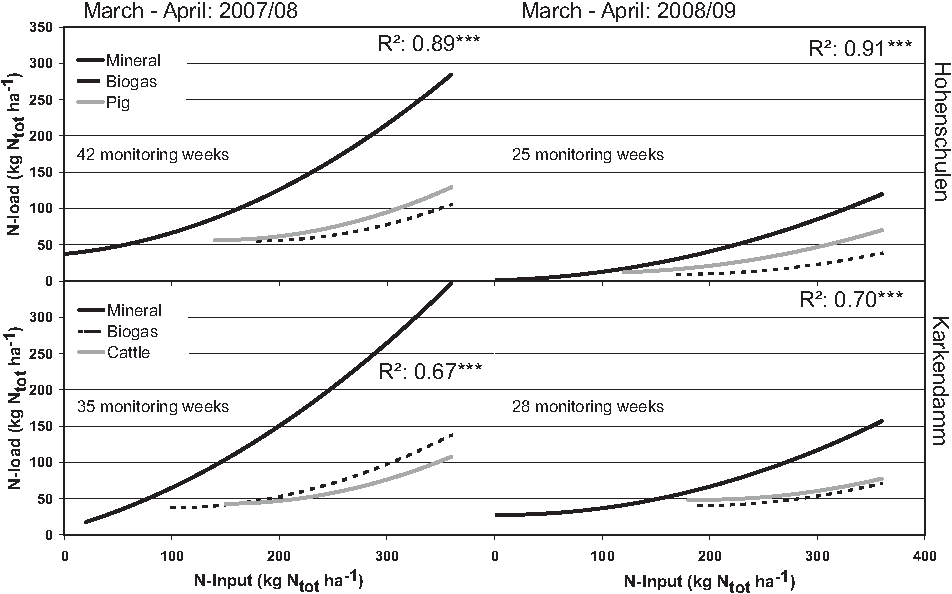
\includegraphics[width=\textwidth]{grafik.pdf}
\captionof{figure}{Relationship of total N input ($kg N ha^{-1}$) and nitrogen load in leachate ($kg N ha^{-1}$) as influenced by fertiliser type.}
\label{fig:niko}
\end{center}

\section*{Conclusion}

Application of biogas residue resulted in N losses comparable to animal
manure. Potential N losses, however, are underestimated since the monitoring
periods did not cover complete years. Therefore, the N balance will be
simulated in a next step to allow N loss calculations over the whole 2-year
period.

%\subsection{References}


\bibliographystyle{plainnat}
\bibliography{niko}

\end{document}
